\chapter{Os Impactos da Reforma Previdenciária Acerca das Concessões de Benefícios de Aposentadoria}

% --------------------------------------------------------------------------- %
\section{Considerações Iniciais}

Conforme demonstrado no capítulo anterior, as aposentadorias e pensões compreendem uma importante categoria na composição de renda da população brasileira, impactando diretamente na desigualdade socioeconômica nacional. Dessa forma, acerca da magnitude social que esses benefícios proporcionam, evidencia-se que alterações nas regras de acesso ao regime previdenciário, como as previstas pela PEC 287/16\footnote{Disponível em: <https://www.camara.leg.br/proposicoesWeb/fichadetramitacao?idProposicao=2119881> Acesso em: 14 Jan, 2020}) ou PEC 6/2019\footnote{Disponível em: <https://www.camara.leg.br/proposicoesWeb/fichadetramitacao?idProposicao=2192459> Acesso em: 14 Jan, 2020}, tendem a apresentar importantes consequências acerca da sociedade. 

Embora diversos trabalhos abordem a sustentabilidade da Previdência Social, estimando projeções econômicas a curto e longo prazo \cite{cap03_ref5, cap05_ref9}, ou a confiabilidade dos resultados divulgados pelo governo para justificar as referidas reformas \cite{cap05_ref10, cap01_ref3}, observa-se na literatura a ausência de pesquisas que investiguem os efeitos que tais alterações nas regras de acesso causariam nas concessões de aposentadorias.

Dessa forma, esse estudo de caso objetivou avaliar os impactos que a reforma prevista pela PEC 06/2019 pode causar no cenário previdenciário brasileiro acerca das concessões dos benefícios de aposentadoria. Especificamente, visou, através de uma abordagem de ciência de dados, utilizar os dados oficiais disponibilizados pela CPI da Previdência, pelo IBGE e pelo Anuário Estatístico da Previdência Social, para simular os efeitos que a PEC 06/2019 causariam no período de 1995 a 2016 se a mesma já estivesse em vigor no momento em que cada benefício foi concedido.

Para isso, esse capítulo foi dividido em 4 subseções incluindo esta breve introdução. Em seguida, na subseção~\ref{cap05:metodologia}, será abordada a metodologia para o desenvolvimento das análises realizadas, evidenciando a arquitetura utilizada para armazenamento dos dados, validação das informações disponibilizadas e detalhes da simulação proposta. Na subseção~\ref{cap05:resultados} serão discutidos os principais resultados encontrados, finalizando o estudo na subseção~\ref{cap05:conclusoes} com as considerações finais. 

% --------------------------------------------------------------------------- %
\section{Metodologia Utilizada}\label{cap05:metodologia}

Para o desenvolvimento do estudo proposto foi estabelecida uma sequência de etapas relacionadas a análise de dados, semelhante ao estudo anterior. No entanto, devido à natureza da problemática, e ao fato da pesquisa necessitar de outras fontes de informações para a abstração de melhores \textit{insights}, foi adotada uma estratégia metodológica diferente. Sendo assim, como forma de otimizar a organização, armazenamento e consultas nos dados, foi elaborado uma estrutura de \textit{Data Warehouse}\footnote{Data warehouse compreende uma organização para banco de dados comumente utilizada em inteligência de negócios. Sua principal característica esta relacionada ao armazenamento de grandes quantidade dados, de diferentes fontes, em uma arquitetura que possibilite a realização de consultas complexas com maior grau de facilidade.} contendo todas as bases de dados inerentes ao estudo. A Figura~\ref{fig:cap05:metodologia} exibe o fluxo de desenvolvimento deste estudo de caso, contendo cada uma das etapas realizadas seguido por um grau de detalhamento mais aprofundado acerca dessa seção.

\begin{figure}[!ht]
    \centering
    \caption{Fluxograma de desenvolvimento do segundo estudo de caso}
    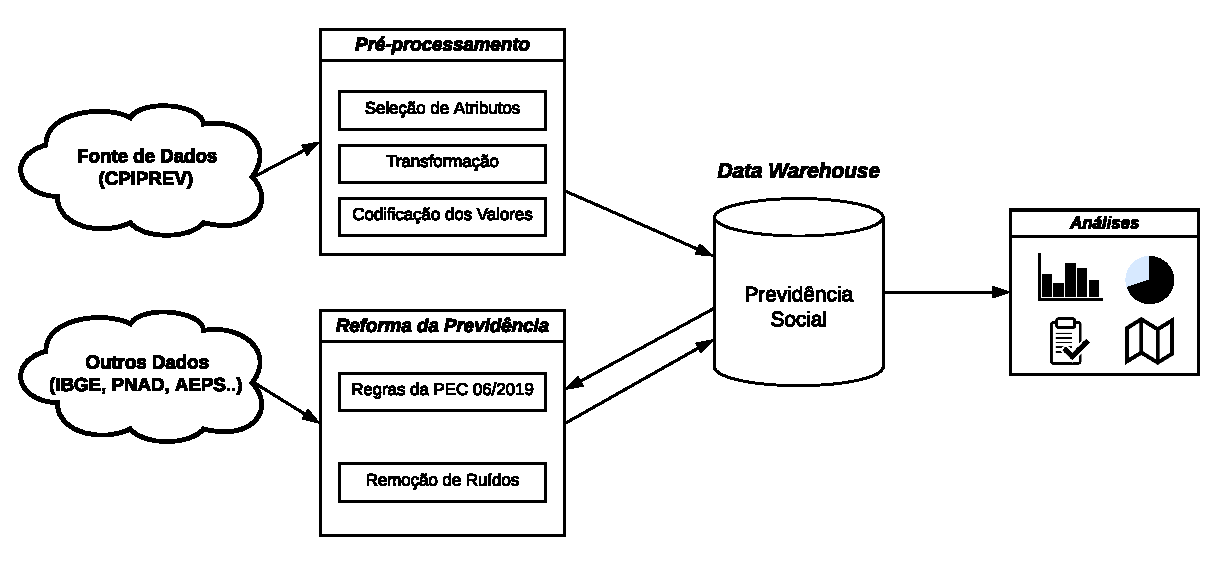
\includegraphics[width=\textwidth]{figs/cap05_metodologia_estudo02.pdf}
    \caption*{\footnotesize{Fonte: Elaborado pelo autor}}
    \label{fig:cap05:metodologia}
\end{figure}

\subsection{Origem dos Dados e Elaboração do \textit{Data Warehouse}}

O estágio inicial do procedimento metodológico deste estudo norteou-se na aquisição dos microdados previdenciários necessários para a reprodução da PEC 06/2019. Sendo assim, após a divulgação do trabalho de \cite{cap05_ref9}, foram solicitadas as informações ausentes nos anexos das LDOs, necessárias para a reprodução dos seus cálculos. Dessa forma, o Ministério da Fazenda disponibilizou os dados referentes a aposentadorias e pensões no site\footnote{Disponível em: <https://legis.senado.leg.br/comissoes/docsRecCPI?codcol=2093> Acesso em: 17 Fev, 2020} CPI da Previdência de 2017, enumerados pelos documentos DOC090 e DOC097.

Esses documentos compreendem séries históricas de dados relacionados a concessão de benefícios de diversas espécies, sendo as principais: aposentadorias por tempo de contribuição (espécie 42), por tempo de contribuição especial (espécies 46 e 57), por idade (espécie 41), por invalidez (espécie 32), além dos benefícios de pensão por morte (espécie 21) e auxílio doença (espécie 31). A Tabela~\ref{tab:cap05:dadosprevidencia} exibe um breve resumo acerca dos dados disponibilizados pela CPI da Previdência de 2017.

\begin{table}[!h]
    \caption{Informações sobre os microdados disponibilizados pela CPI da Previdência de 2017.}
    \resizebox{\textwidth}{!}{
  \begin{tabular}{|cc|c|c|}
    \hline
    \multicolumn{1}{|c|}{\textbf{Origem}} & \textbf{Arquivos} & \textbf{Nº de Registros} & \textbf{Descrição} \\ \hline
    \multicolumn{1}{|c|}{\multirow{2}{*}{DOC090}} & APOSENTADORIAS.csv & 46.545.767 & \begin{tabular}[c]{@{}c@{}}Benefícios de Aposentadorias \\ (42, 46, 57, 41 e 32) e Auxílio 31 \\ concedidos entre 2000 e 2015\end{tabular} \\ \cline{2-4} 
    \multicolumn{1}{|c|}{} & PENSAO.csv & 5.647.457 & \begin{tabular}[c]{@{}c@{}}Benefícios de Pensão da espécie 21\\ concedidas entre 2000 e 2015\end{tabular} \\ \hline
    \multicolumn{1}{|c|}{\multirow{2}{*}{DOC097}} & SEN\_MICRODADOS01.APO.AUX.csv & 57.955.872 & \begin{tabular}[c]{@{}c@{}}Benefícios de Aposentadorias \\ (42, 46, 57, 41, 32 e 92) e Auxílios\\ (91 e 31) concedidos entre 1995 e 2016\end{tabular} \\ \cline{2-4} 
    \multicolumn{1}{|c|}{} & SEN\_MICRODADOS02\_PENS.csv & 7,964,185 & \begin{tabular}[c]{@{}c@{}}Benefícios de Pensão por Morte\\ (21, 93) concedidos entre 1995 e 2016\end{tabular} \\ \hline
     &  & \textbf{118.113.281} &  \\ \hline
  \end{tabular}}
    \label{tab:cap05:dadosprevidencia}
    \caption*{\footnotesize{Fonte: Elaborado pelo autor.}}
\end{table}

Para a realização das análises e simulações propostas, optou-se por utilizar o arquivo SEN\_MICRODADOS01.APO.AUX.csv devido ao fato desse agregar informações relacionadas às principais espécies de aposentadorias em um maior intervalo de tempo. Assim sendo, a base de dados foi inserida na estrutura de \textit{Data Warehouse} dividindo a base de dados em diferentes tabelas do tipo FATO e DIMENSAO, sendo as primeiras responsáveis pelo conteúdo bruto dos dados (registros de aposentadorias) e as segundas por dados complementares (formato de datas, espécies de aposentadorias, tipo de clientela, etc) utilizadas principalmente em consultas mais específicas e complexas.

Para a elaboração da estrutura da \textit{Data Warehouse} e bancos de dados, além da criação das tabelas FATO e DIMESAO e conversão dos dados contidos no arquivo .csv (\textit{comma separated values}) em registros, foi utilizado o \textit{software} de código aberto \textit{Pentaho Data Integration} (PDI)\footnote{Disponível em: <https://community.hitachivantara.com/s/article/data-integration-kettle> Acesso em: 18 Fev, 2020}. Devido ao fato dessa ferramenta ser fortemente utilizada na área de inteligência de negócios, a mesma promove um conjunto de funcionalidades relacionadas a análise de dados tais como suporte à linguagem Structured Query Language (SQL) e comunicação com os principais sistemas gerenciadores de bancos de dados. 

Diante disso, foram utilizadas funcionalidades do PDI e da linguagem de programação SQL para realizar uma etapa de pré-processamento dos dados. Essa etapa compreendeu a seleção dos atributos relevantes para o estudo e transformações acerca dos microdados, como por exemplo codificação de valores textuais em numéricos para diminuir a demanda computacional necessária. Por fim, os microdados resultantes, correspondentes a série histórica de benefícios de aposentadorias/auxílios concedidos entre os anos de 1995 e 2016, foram armazenados em SGBD PostgreSQL. O Apêndice~\ref{apendice:a} apresenta, resumidamente, os principais metadados presentes nesta base de dados, podendo ser encontrado ao final deste documento.
	
Diante disso, a partir da utilização de funcionalidades do PDI e da linguagem de programação SQL, foi realizada uma etapa de pré-processamento dos dados, a qual compreendeu a seleção dos atributos relevantes para o estudo e transformações acerca dos microdados, como a codificação dos valores textuais em numéricos. Posteriormente, os dados resultantes, correspondentes a série histórica de benefícios de aposentadorias/auxílios concedidos entre os anos de 1995 e 2016, foram armazenados em um SGBD PostgreSQL.

Destaque-se que a utilização de uma estrutura de \textit{Data Warehouse} não possibilita a inserção ou remoção de registros no banco de dados de maneira automática e dinâmica. Para tal funcionalidade, o administrador da arquitetura – utilizando técnicas de \textit{Extract, Transfom and Load} (ETL) responsáveis por extrair, transformar/pré-processar e carregar dados de diferentes origens em bancos de dados – promove a atualização do \textit{Data Warehouse} de acordo com a demanda necessária \cite{cap05_ref12, cap05_ref13}. Todavia, devido à natureza da aplicação realizada nesse estudo não promover uma atualização dinâmica nos dados, fator justificado pela dificuldade de acesso a microdados recentes de concessões de aposentadorias, essa ferramenta apresentou-se promissora uma vez que possibilita consultas mais complexas e com menor grau de dificuldade.  

\subsection{Análise Exploratória}

Uma vez que o desenvolvimento do \textit{Data Warehouse} responsável pelo armazenamento dos microdados previdenciários foi realizado, constatou-se a necessidade de efetuar uma análise exploratória acerca dos dados, objetivando, principalmente, compreender o seu conteúdo e avaliar a confiabilidade das informações disponibilizadas. Dessa forma, foram utilizados os microdados fornecidos pelo DATAPREV para recalcular os resultados divulgados pelo Anuário Estatístico da Previdência Social (AEPS)\footnote{O AEPS foi criado em 1992 e é responsável por disponibilizar para a populações dados estatísticos e básicos referentes a situação dos benefícios mantidos pelo INSS e sobre suas arrecadações de contribuições previdenciárias \cite{cap05_ref14}}. Inicialmente foi elaborada uma série histórica comparativa referentes a concessão dos benefícios de aposentadorias. A Figura~\ref{fig:cap05:aepsvsprev}(a) ilustra o comportamento de ambas as fontes de dados para o intervalo de 1995-2016. Por sua vez, a Figura~\ref{fig:cap05:aepsvsprev}(b) exibe o erro percentual existente entre as duas, enfatizando o ano de 1995, o que apresentou uma diferença acima de 8\% entre dados disponibilizados pela CPI e o AEPS daquele ano.

\begin{figure}[!ht]
    \centering
    \caption{(a) Comparação entre os dados disponibilizados pela CPI da Previdência e as informações contidas no APES. (b) Erro percentual.}
    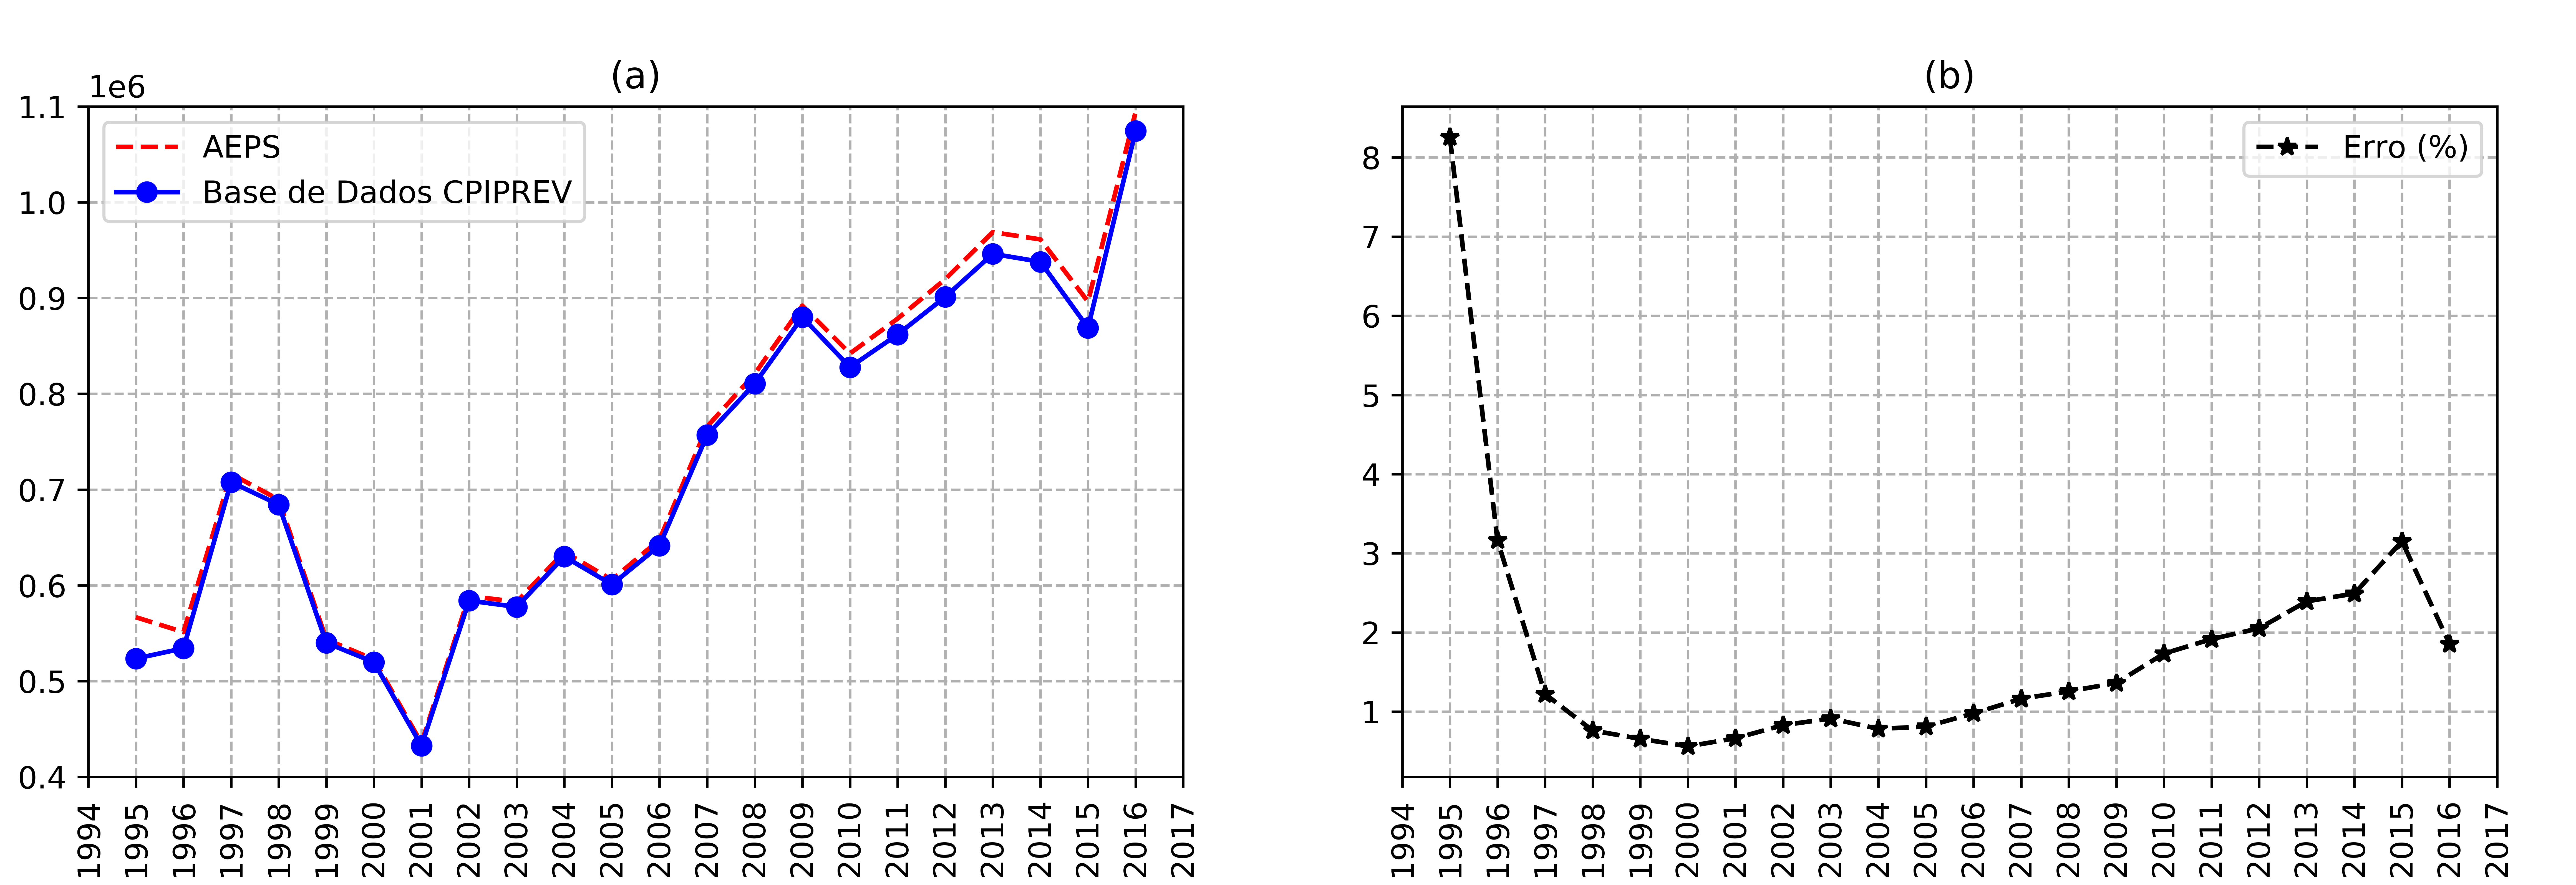
\includegraphics[width=\textwidth]{figs/cap05_apes_vs_cpiprev.png}
    \caption*{\footnotesize{Fonte: Elaborado pelo autor}}
    \label{fig:cap05:aepsvsprev}
\end{figure}

Similarmente, foi reproduzido um dos resultados contidos no AEPS de 2016, intitulado "A.1 - Quantidade de benefícios concedidos, por clientela, segundo os grupos de espécies - 2014/2016", contido na página 21\footnote{Disponível em: <http://sa.previdencia.gov.br/site/2018/08/aeps2016.pdf> Acesso em: 5 de Mar, 2020}, utilizando os microdados disponibilizados pelo DATAPREV. Com isso, conforme exibido na Tabela~\ref{fig:cap05:comparacaoaposen}, notou-se uma pequena variação entre os resultados, proveniente, possivelmente, de ações jurídicas relacionadas a concessões de benefícios, ou seja, contribuintes que deram entrada em benefícios e tiveram retorno após a data de disponibilização dos dados pela CPI da previdência. 

\begin{table}[!h]
    \caption{Comparação entre os dados disponibilizados pelo DATAPREV e as informações contidas no APES: Quantidade de benefícios concedidos por grupos de espécies entre 2014/2016}
    \resizebox{\textwidth}{!}{
    \begin{tabular}{|l|c|c|c|c|c|c|}
        \hline
        \multicolumn{1}{|c|}{\multirow{2}{*}{\textbf{Espécie}}} & \multicolumn{3}{c|}{\textbf{AEPS}} & \multicolumn{3}{c|}{\textbf{DATAPREV}} \\ \cline{2-7} 
        \multicolumn{1}{|c|}{} & \textbf{2014} & \textbf{2015} & \textbf{2016} & \textbf{2014} & \textbf{2015} & \textbf{2016} \\ \hline
        Aposentadorias & 1.150.880 & 1.058.151 & 1.263.974 & 1.115.107 & 1.058.379 & 1.290.267 \\ \hline
        - Tempo de Contribuição & 315.542 & 320.460 & 432.033 & 315.483 & 320.414 & 439.850 \\ \hline
        - Idade & 645.687 & 575.841 & 662.366 & 645.744 & 575.886 & 674.338 \\ \hline
        - Invalidez & 189.651 & 161.850 & 169.575 & 189.880 & 162.079 & 176.079 \\ \hline
    \end{tabular}}
    \caption*{\footnotesize{Fonte: Elaborado pelo autor}}
    \label{fig:cap05:comparacaoaposen}
\end{table}

Posteriormente, após validar a confiabilidade dos dados utilizados, foi estimada a quantidade de registros existentes na base de dados classificando-os por espécies de benefícios. Dessa forma, a Figura~\ref{fig:cap05:percentapo} exibe um gráfico de barras contendo os percentuais de participação de cada categoria na base de dados, enfatizando as aposentadorias das espécies 42, 46, 57, 41, 32 e 92 (34,62\% do total) correspondentes aos benefícios diretamente atingidos pela reforma previdenciária prevista na PEC 06/2019.

\begin{figure}[!h]
    \centering
    \caption{Percentual de participação dos benefícios da base dados classificados por espécie.}
    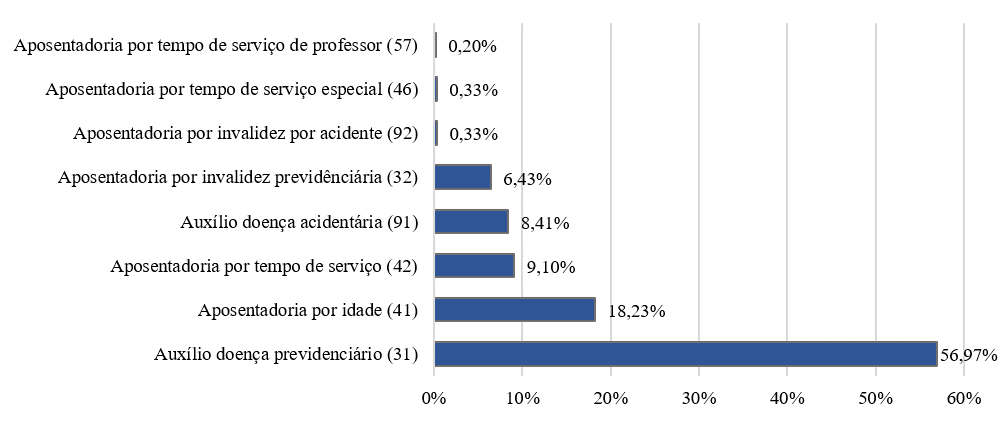
\includegraphics[width=\textwidth]{figs/cap05_percentual_especies.png}
    \caption*{\footnotesize{Fonte: Elaborado pelo autor}}
    \label{fig:cap05:percentapo}
\end{figure}

Em contrapartida, quando analisada a proporção de aposentadorias concedidas classificando-as por sexo, identificou-se relativo grau de equilíbrio com 55,06\% dos segurados correspondendo ao sexo masculino, 44,93\% ao feminino e 0,01\% com o sexo ignorado/indefinido. No entanto, devido a natureza das simulações propostas, a última categoria foi desconsiderada visto que as regras previstas na PEC 06/2019 não incorporavam diretrizes relacionadas a sexo indefinido. 

Após a realização da análise exploratória e validação das informações existentes no banco de dados, contatou-se a possibilidade de simular a reforma da previdenciária conforme previsto nos objetivos deste estudo. Além disso, outras análises estatísticas e quantitativas mais detalhadas foram realizadas a fim de compreender melhor o conteúdo desses microdados. Foram disponibilizadas as informações referentes a essas análises complementares, a documentação necessária para sua replicação os códigos fontes utilizados para cada cálculo e consulta realizados acerca da base de dados no repositório do projeto disponível na plataforma GitHub\footnote{Disponível em: <https://github.com/andrespp/ds-prev> Acesso em: 3 Mai, 2020}.

\subsection{Simulação da Reforma Previdenciária (PEC06/2019)}

Após a realização das etapas anteriores, e utilizando dados públicos disponibilizados pelo IBGE e AEPS, foi elaborada e incorporada uma nova base de dados ao \textit{Data Warehouse} referente a uma simulação das regras previstas pela reforma da previdência prevista na PEC 06/2019\footnote{As regras utilizadas são referentes à proposta em vigor no dia 15/06/2019, podendo eventualmente ter sofrido alterações após a publicação do trabalho.}. A Tabela~\ref{fig:cap05:regraspec} exibe de forma resumida as diretrizes previstas pela reforma para as principais espécies de benefícios em relação a idade mínima e tempo de contribuição em anos. 

\begin{table}[!h]
    \centering
    \caption{Regras para obtenção de aposentadorias propostas pela PEC 06/2019.}
    \newcolumntype{P}[1]{>{\centering\arraybackslash}p{#1}}
    \begin{tabular}{|P{3cm}|P{2.2cm}|P{2.2cm}|P{2.2cm}|P{2.2cm}|}
    \hline
    \multirow{2}{*}{\textbf{Espécie}} & \multicolumn{2}{c|}{\textbf{Idade}} & \multicolumn{2}{c|}{\textbf{Tempo de Contribuição}} \\ \cline{2-5} 
     & \textbf{Mulher} & \textbf{Homem} & \textbf{Mulher} & \textbf{Homem} \\ \hline
    Urbana (41/42) & 62 & 65 & 15 & 20 \\ \hline
    Rural (41/42) & 55 & 60 & \multicolumn{2}{c|}{15} \\ \hline
    Professor (57) & 57 & 60 & \multicolumn{2}{c|}{25} \\ \hline
    Especial (46) & \multicolumn{2}{c|}{55} & \multicolumn{2}{c|}{15} \\ \hline
    Especial (46) & \multicolumn{2}{c|}{58} & \multicolumn{2}{c|}{20} \\ \hline
    Especial (46) & \multicolumn{2}{c|}{60} & \multicolumn{2}{c|}{25} \\ \hline
    \end{tabular}
    \caption*{\footnotesize{Fonte: Elaborado pelo autor}}
    \label{fig:cap05:regraspec}
\end{table}

Essa nova base de dados, além de compreender o universo de registros existentes no banco de dados da previdência, agrega novos atributos referentes a projeções de como tais benefícios se comportariam caso a reforma já estivesse em vigor no momento em que cada aposentadoria foi concedida\footnote{A simulação não considera regras de transição, mas sim as regras finais para concessão de cada benefício.}. Na Figura~\ref{fig:cap05:fluxograma} é possível visualizar, de forma resumida, a lógica utilizada para a realização da simulação proposta através de um fluxograma, o qual terá um maior grau de detalhamento das tarefas realizadas no decorrer desta subseção. 

\newpage

\begin{figure}[!h]
    \centering
    \caption{Fluxograma da simulação da reforma previdenciária PEC 06/2016}
    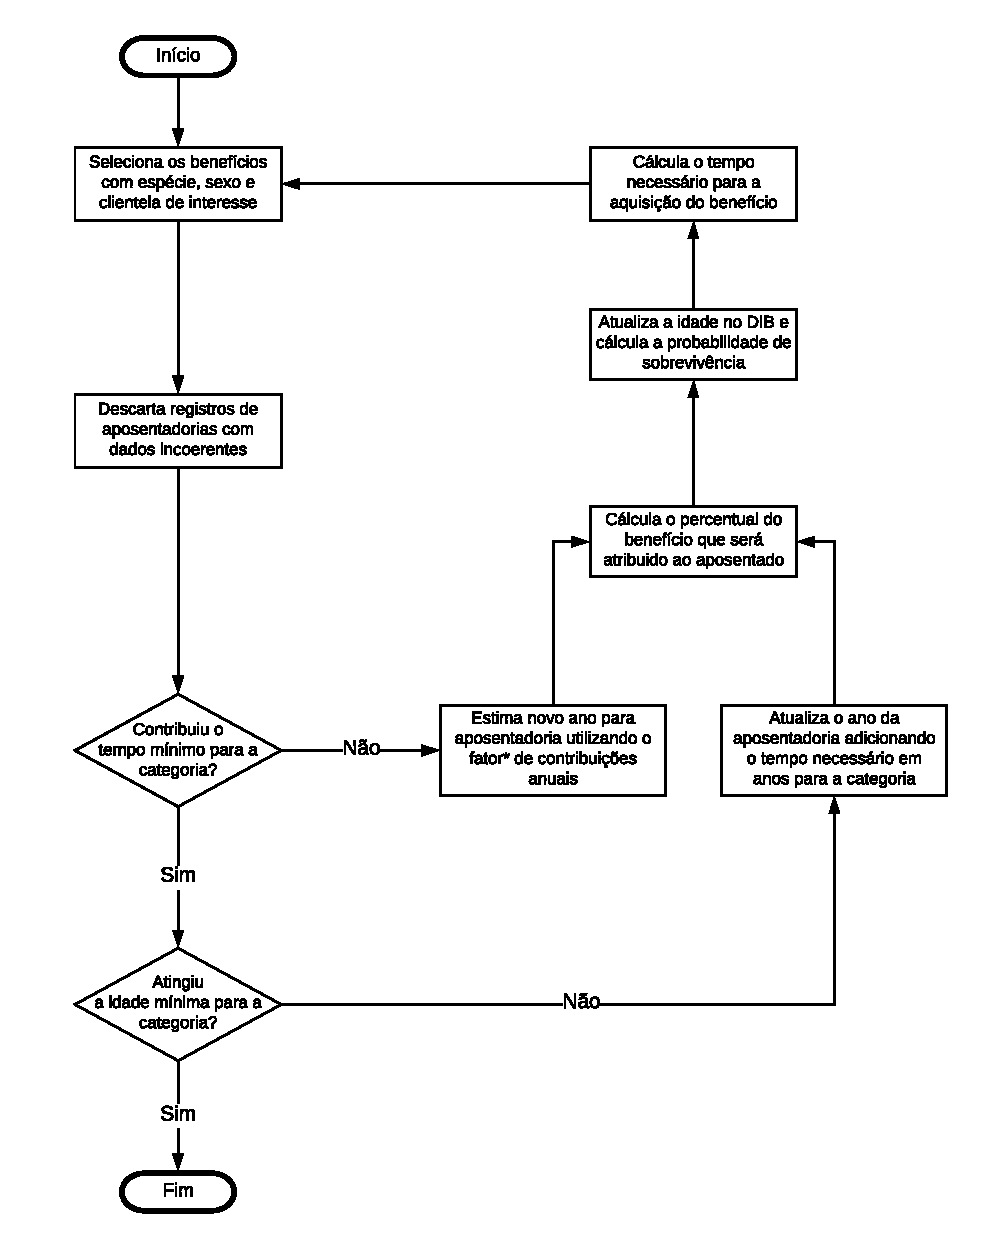
\includegraphics[width=\textwidth]{figs/cap05_fluxograma_reforma_previdencia.pdf}
    \caption*{\footnotesize{Fonte: Elaborado pelo autor}}
    \label{fig:cap05:fluxograma}
\end{figure}

\noindent* O fator de contribuições anuais, destacado no fluxograma, corresponde ao número médio de contribuições anuais, em meses, realizado por cada beneficiário.

\newpage

Inicialmente, houve a leitura e seleção dos registros inerentes a pesquisa, correspondendo aos benefícios das espécies 41, 42, 46, 57, 32 e 92 – aposentadorias por idade, tempo de contribuição, tempo de contribuição especial, tempo de contribuição professor, invalidez previdenciária e invalidez acidentária, respectivamente – para os gêneros masculino e feminino, com clientela urbana e rural, os quais corresponderam a 19.775.373 registros da base de dados. Entretanto, devido a existência de anomalias na idade e tempo de contribuição dos beneficiários, houve uma etapa de triagem nos microdados, reduzindo o universo de interesse em aproximadamente 12,84\% em relação a quantidade anterior, resultando em 17.236.900 registros válidos. 

Após a seleção e remoção de ruídos nos dados de interesse, foram realizadas as simulações propostas. Diante disso, primeiramente, foi verificado se o tempo de contribuição de cada beneficiário correspondia ao tempo mínimo em anos necessário para que a sua categoria obtivesse acesso ao benefício. Caso sim, o registro era selecionado para a próxima etapa, no entanto, caso não, seria estimado e agregado ao beneficiário o tempo em anos necessário para que o mesmo atingisse a regra proposta. Para tal estimativa, levou-se em consideração a dificuldade dos trabalhadores do setor privado se manterem em seus respectivos trabalhos devido, principalmente, as altas taxas de desemprego e informalidade existentes no país \cite{cap04_ref5}. Em seguida, verificou-se se cada beneficiário atingia a idade mínima da sua categoria para a concessão da aposentadoria, acrescentando o tempo a mais que o mesmo haveria de esperar para ter acesso a seu benefício quando necessário.

Dessa forma, após estimar as novas idades e tempo a mais de contribuição, foram calculadas as probabilidades dos beneficiários que não atendiam as regras previstas na PEC 06/2019 estarem vivos na futura concessão dos seus benefícios. Para isso, optou-se por utilizar a projeção populacional realizada pelo IBGE, a qual corresponde a dados de estimativas demográficas a nível nacional classificadas por sexo, idade e clientela, de 2010 a 2060. Assim sendo, a probabilidade de sobrevivência de cada beneficiário pode ser calculada através da Equação~\ref{eq:5.1} abaixo.

\begin{equation}
    prob\_sobrev(i_{proj}, a_{proj}, s) = \frac{POP\_proj(i_{proj}, a_{proj}, s)}{POP\_atual(i_{atual}, a_{atual}, s)}, \left \{a \epsilon \mathbb{I} | 2010 \leq a \leq 2060 \right \}
    \label{eq:5.1}
\end{equation}

\noindent sendo $s$ o sexo do beneficiário e, $i_{proj}$, $i_{atual}$, $a_{proj}$ e $i_{atual}$ a idade na projeção, idade atual, ano na projeção e ano atual, receptivamente. Além disso, as variáveis $POP\_atual$ e $POP\_projetada$ correspondem as populações atuais e projetadas pelo IBGE para cada idade, sexo e ano de interesse.

Por fim, foi calculado o percentual a ser aplicado na média dos salários (contribuições) de cada beneficiário baseando-se nas regras previstas pela reforma da previdência, a qual estipula uma mensalidade 60\% do valor médio, possibilitando um acréscimo de 2\% para cada ano que exceder o tempo mínimo de contribuição . Dessa forma, foram criados sete novos atributos correspondentes a simulação da PEC 06/2019, sendo:

\begin{itemize}
    \item \texttt{PEC6\_GAP\_IDADE}: quantidade de anos a mais que o beneficiário deveria esperar para obter o benefício considerando as novas regras;
    
    \item \texttt{PEC6\_GAP\_CONTRIB}: quantidade de anos a mais que o beneficiário deveria trabalhar para obter o benefício considerando as novas regras;
    
    \item \texttt{PEC6\_GAP}: valor máximo entre o \texttt{PEC6\_GAP\_IDADE} e \texttt{PEC6\_GAP\_CONTRIB};
    
    \item \texttt{PEC6\_ANO\_DIB}: ano mínimo em que o beneficiário terá acesso ao benefício considerando as novas regras;
    
    \item \texttt{PEC6\_IDADE\_DIB}: idade do beneficiário na nova data de início do benefício de aposentadoria considerando as novas regras;
    
    \item \texttt{PEC6\_PROB}: probabilidade de o beneficiário estar vivo no ano em que ficaria elegível para obtenção do benefício;
    
    \item \texttt{PEC6\_PERCENT}: percentual a ser aplicado sobre a média das contribuições para fins de cálculo do valor do benefício.
\end{itemize}

Para o desenvolvimento dessa simulação foi utilizada a linguagem de programação \textit{Python 3}, os \textit{frameworks} de análise de dados \textit{Pandas} e \textit{Numpy} e biblioteca \textit{Psycopg2} responsável por estabelecer uma conexão com o banco de dados PostgreSQL. No repositório do projeto, disponibilizado através da plataforma GitHub\footnote{Disponível em: <https://github.com/andrespp/ds-prev> Acesso em: 3 de Mai, 2020}, pode-se encontrar os \textit{scripts} utilizados em toda simulação com toda a documentação necessária para sua reprodução, apresentando dessa forma um maior grau de detalhamento acerca dos cálculos realizado para cada novo atributo. A Tabela~\ref{tab:cap05:github} descreve a estrutura do projeto e os principais arquivos existentes.

\newpage

\begin{table}[!h]
    \centering
    \caption{Descrição dos principais arquivos do projeto no GitHub referente ao segundo estudo de caso} 
    \begin{tabular}{p{0.22\textwidth}p{0.6\textwidth}}
    \hline
    \textbf{requirements.txt} & arquivo de texto descrevendo todas as dependências e pacotes Python necessários para a execução do projeto.\vspace{3mm}            \\
    \textbf{dataset}          & pasta contendo todos os dados necessários para a execução das análises.\vspace{3mm}                                                \\
    \textbf{doc}              & pasta contendo documentos inerentes a simulação, tais como APES, Ofícios da CPI da Previdência, Taxas, dentre outros. \vspace{3mm} \\
    \textbf{compose}          & pasta contendo os arquivos necessários para levantar a infraestrutura do projeto utilizando a aplicação Docker. \vspace{3mm}       \\
    \textbf{metadata}         & pasta contendo os dicionários e documentações das bases de dados.\vspace{3mm}                                                      \\
    \textbf{dw}               & pasta contendo os arquivos necessários para a criação do data warehouse e realização da simulação.\vspace{3mm}                     \\
    \textbf{analisys}         & pasta com as diversas análises realizadas utilizando a \textit{framework jupyter notebook}.\vspace{3mm}                            \\          
    \textbf{README.md}        & descrição das características e funcionamento do projeto.                                                                           \\\hline
    \end{tabular}
    \caption*{\footnotesize{Fonte: Elaborado pelo autor.}}
    \label{tab:cap05:github}
\end{table}

\newpage

\section{Resultados e Discussão}\label{cap05:resultados}

A partir da estruturação e implementação da arquitetura do \textit{Data Warehouse} para o armazenamento dos microdados previdenciários, e aplicando técnicas/estratégias de ciência de dados para a extração de conhecimento válido acerca da problemática abordada, foi possível realizar a simulação proposta nos objetivos desse estudo. Em vista disso, avaliando as atuais diretrizes do sistema previdenciário nacional, observa-se que as duas principais informações utilizadas para avaliar a viabilidade de um contribuinte se aposentar, tanto no regime atual quanto nas regras da PEC 06/2019, consistem na idade da pessoa e do seu tempo de contribuição para o RGPS. A partir dessas informações, e dependendo das características do trabalho exercido pela contribuinte em questão (trabalhador rural ou urbano, do sexo feminino ou masculino, do tipo professor ou não, dentre outros), este pode passar a ter direito ao benefício da sua aposentadoria.

Dessa forma, como ponto de partida para as análises realizadas, e utilizando os dados reais de aposentadorias concedidas no período analisado , calculou-se a idade média de entrada nos benefícios e o tempo médio em anos de contribuições dos aposentados para o intervalo de tempo analisado, exibindo os resultados nas Tabelas~\ref{tab:cap05:idademedia} e \ref{tab:cap05:contribmedia}. Assim, destaca-se que, de forma geral, os homens se aposentavam em média com 58,24 anos de idade contribuindo com 26,77 anos de trabalho, enquanto as mulheres aposentavam-se com 57,23 anos de idade com uma média de 20,57 anos de trabalho contribuídos para a previdência social. 

\begin{table}[!h]
\centering
\caption{Idade média de entrada em benefício pelas regras atuais do RGPS.}
\renewcommand{\arraystretch}{1.2}
 \newcolumntype{P}[1]{>{\centering\arraybackslash}p{#1}}
\begin{tabular}{P{2cm}P{2cm}P{2cm}P{2cm}P{2cm}P{2cm}}
\toprule[2pt]
 & \textbf{Idade} & \textbf{T.C.} & \textbf{T.C. Esp.} & \textbf{Professor} & \textbf{Rural} \\ \hline
\textbf{Homens} & 65,81 & 53,53 & 48,84 & 56,00 & 60,84 \\ \hline
\textbf{Mulheres} & 61,58 & 51,37 & 49,16 & 50,66 & 56,99 \\ \toprule[2pt]
\end{tabular}
\caption*{\footnotesize{Elaborado pelo autor.}}
\label{tab:cap05:idademedia}
\end{table}

\begin{table}[!h]
\centering
\caption{Tempo (em anos) médio de contribuição pelas regras atuais do RGPS.}
\renewcommand{\arraystretch}{1.2}
 \newcolumntype{P}[1]{>{\centering\arraybackslash}p{#1}}
\begin{tabular}{P{2cm}P{2cm}P{2cm}P{2cm}P{2cm}P{2cm}}
\toprule[2pt]
& \textbf{Idade} & \textbf{T.C.} & \textbf{T.C. Esp.} & \textbf{Professor} & \textbf{Rural} \\ \hline
\textbf{Homens} & 20,35 & 34,52 & 26,02 & 30,90 & 18,39 \\ \hline
\textbf{Mulheres} & 17,27 & 29.37 & 25,86 & 26,55 & 17,82 \\ \hline \toprule[2pt]
\end{tabular}
\caption*{\footnotesize{Elaborado pelo autor.}}
\label{tab:cap05:contribmedia}
\end{table}

Avaliando as Tabelas~\ref{tab:cap05:idademedia} e \ref{tab:cap05:contribmedia}, observa-se que, na média, os homens e mulheres que deram entrada em seus benefícios atendiam as regras expostas na Tabela~\ref{fig:cap05:regraspec}. No entanto, é importante evidenciar que nem todos os trabalhadores que se aposentaram por idade, por exemplo, possuíam o tempo mínimo de contribuição previsto nas regas da PEC 06/2019. Dessa forma, destaca-se que esse período faltando não compreende necessariamente o tempo de trabalho adicional que, na prática, esses contribuintes teriam que cumprir para se aposentarem. Tal fator é justificado pelas elevadas taxas de desemprego e informalidade que impactam diretamente na estabilidade dos trabalhadores do setor privado, dificultando que os mesmos trabalhem formalmente de forma ininterrupta, e consequentemente implicando na idade que estes iriam se aposentar.

Sendo assim, estima-se que os homens aposentados por idade pelas regras atuais necessitariam trabalhar um tempo adicional maior que o previsto, aplicando a mesma analogia para as mulheres e para os demais tipos de aposentadorias consideradas nessa pesquisa. Com isso, utilizando as informações disponibilizadas pelas Tabelas~\ref{tab:cap05:idademedia} e \ref{tab:cap05:contribmedia}, e partindo do princípio de que todos começaram a trabalhar com 18 anos, foi calculado o número médio de contribuições\footnote{Idealmente, o número médio de contribuições por ano deveria ser igual a 12, correspondente a 12 meses de trabalho.} por ano para cada espécie de aposentadoria avaliada, tendo os resultados exibidos na Tabela~\ref{tab:cap05:numcontrib}.

\begin{table}[!h]
\centering
\caption{Número médio de contribuições por ano.}
\renewcommand{\arraystretch}{1.2}
 \newcolumntype{P}[1]{>{\centering\arraybackslash}p{#1}}
\begin{tabular}{P{2cm}P{2cm}P{2cm}P{2cm}P{2cm}P{2cm}}
\toprule[2pt] 
 & \textbf{Idade} & \textbf{T.C.} & \textbf{T.C. Esp.} & \textbf{Professor} & \textbf{Rural} \\ \hline
\textbf{Homens} & 5.11 & 11,66 & 10,13 & 9,76 & 5,15 \\ \hline
\textbf{Mulheres} & 4,76 & 11,57 & 9,96 & 9,76 & 5.49 \\ \hline \toprule[2pt]
\end{tabular}
\caption*{\footnotesize{Fonte: Elaborado pelo autor.}}
\label{tab:cap05:numcontrib}
\end{table}

Tais resultados demonstram que, pelas regras previstas na PEC 06/2019, em algumas situações, o tempo de contribuição necessário para se aposentar, em média, chegaria a equivaler ao dobro do tempo de contribuição restante. Por exemplo, um homem com 65 anos de idade e 15 anos de contribuição, que nas regras atuais consegue a concessão de aposentadoria por idade mas não atende as regras da PEC 06/2019 pela necessidade de 5 anos extras de contribuição, necessitaria trabalhar em média 11,74 anos a mais, visto que a cada ano o mesmo só conseguiria contribuir com 5,11 parcelas, resultando em uma idade de aproximadamente 77 anos ao se aposentar.

Além disso, é importante esclarecer que o número médio de contribuições anuais pode variar de acordo com o cenário econômico vivenciado pelo trabalhador. Crises econômicas e elevações nas taxas de desemprego e informalidade tendem a diminuir as contribuições realizadas, gerando, consequentemente, aumento no tempo adicional de trabalho para as concessões dos benefícios de acordo com as regras da PEC 06/2019.

Paralelamente, uma vez que há modificações nas regras para admissão dos beneficiários, evidencia-se alterações no cenário previdenciário em relação a concessões de aposentadorias. Em geral, as diretrizes atuais especificam que os trabalhadores devem possuir uma idade mínima ou ter um tempo de contribuição mínimo para que o benefício possa ser obtido. Uma vez que as regras propostas pela reforma conciliam ambos os critérios como pré-requisitos para obtenção da aposentadoria, estima-se que uma grande parcela dessas pessoas, possivelmente, não conseguiria mais se aposentar na mesma época em que se aposentou pelas regras atuais.  

Diante disso, utilizando os microdados previdenciários e estratégias computacionais para análises em grandes quantidades de dados\footnote{Devido ao fato da base de dados possuir um volume de informações maior que a quantidade de memória tipicamente disponível em um computador doméstico, optou-se por um processamento em lotes, onde subconjutos dos dados de tamanhos compatíveis com os recursos computacionais disponíveis foram processados sequencialmente.}, foi estimado o percentual de aposentados que teriam acesso aos seus benefícios perante as novas regras propostas. Dessa forma, constatou-se que aproximadamente 83,28\% dos trabalhadores que tiveram suas aposentadorias concedidas durante o intervalo de tempo analisado não teriam acesso a esses benefícios caso a reforma estivesse em vigor desde 1995. A Tabela~\ref{tab:cap05:proporcao} apresenta a proporção de aposentadorias concedidas entre 1995 e 2016 que não atendem as regras pela PEC 06/2019, classificando-as de acordo com seus respectivos sexos, clientelas e espécies do benefício obtido.

\begin{table}[!h]
\centering
\caption{Proporção de pessoas que não atendem as regras da PEC na mesma data que deram entrada nos benefícios com as regras atuais.}
\renewcommand{\arraystretch}{1.2}
 \newcolumntype{P}[1]{>{\centering\arraybackslash}p{#1}}
\begin{tabular}{P{2cm}P{2cm}P{2cm}P{2cm}P{2cm}P{2cm}}
\toprule[2pt] 
 & \textbf{Idade} & \textbf{T.C.} & \textbf{T.C. Esp.} & \textbf{Professor} & \textbf{Rural} \\ \hline
\textbf{Homens} & 51,29\% & 98,57\% & 96,88\% & 77,89\% & 55,77\% \\ \hline
\textbf{Mulheres} & 84,27\% & 98,90\% & 97,91\% & 86,18\% & 87,13\% \\ \toprule[2pt]
\end{tabular}
\caption*{\footnotesize{Fonte: Elaborado pelo autor.}}
\label{tab:cap05:proporcao}
\end{table}

Assim, dos homens que se aposentaram por idade, 51,29\% não teriam conseguido o benefício, enquanto para as mulheres, das que se aposentaram por idade, 84,27\% não teriam conseguido se aposentar. A mesma leitura é aplicada para as pessoas que se aposentaram nas espécies de Aposentadoria por Tempo de Contribuição, Aposentadoria por Tempo de Contribuição Especial, Aposentadoria de Professor e Aposentadoria Rural. Além disso, analisando os resultados, constata-se que as mulheres são as mais impactadas em todas as categorias. Tal fator ocorre, principalmente, devido ao acréscimo na idade mínima – de 60 para 62 anos – necessária para que as pessoas do sexo feminino possam ter acesso aos seus benefícios.

Paralelamente, avaliando os resultados da simulação relacionados ao tempo médio adicional de trabalho, ou espera, necessários para a obtenção da aposentadoria daqueles que não cumpriram as regras previstas na PEC, considerando todo o período de 1995 a 2016, observa-se a existência de duas possíveis situações: (i) pessoas que não atingiram a idade mínima, mas já cumpriram o tempo mínimo de contribuição; (ii) 

Na primeira situação, temos os trabalhadores que pelas regras atuais obtiveram o benefício da aposentadoria por tempo de contribuição, incluindo os professores que se aposentaram com idade inferior à proposta pela PEC 06/2019. Neste caso, estes trabalhadores necessitariam apenas esperar a idade mínima necessária sem a exigência de continuar contribuindo para a previdência social. Com isso, estimou-se que os homens que se aposentaram por tempo de contribuição deveriam em média esperar aproximadamente mais 11,18 anos até alcançarem a idade mínima, enquanto as mulheres mais 10,31 anos. No caso dos professores e professoras, haveria a necessidade de aguardar em média 5,15 a 7,19 anos, respectivamente. Embora não seja obrigatoriamente exigido que essas pessoas continuassem trabalhando e contribuindo para alcançarem a aposentadoria, provavelmente as mesmas iriam, em detrimento da necessidade de arcar com sua subsistência.

Por outro lado, na segunda categoria encontram-se, no geral, as pessoas que, pelas regras atuais, aposentam-se por idade, incluindo praticamente 100\% dos trabalhadores rurais. Nessa situação específica, é obrigatório que os trabalhadores continuem contribuindo para o sistema previdenciário até cumprirem os requisitos exigidos pela PEC. Desse modo, observa-se que os homens urbanos e rurais que alcançaram os requisitos mínimos para a aposentadoria por idade pelas regras atuais, necessitariam trabalhar, em média, aproximadamente 4,80 e 6,20 anos a mais, respectivamente. Já para as mulheres, haveria a necessidade de acréscimo médio de 3,31 anos no setor urbano e 4,55 anos no rural. Acerca disso, a Tabela~\ref{tab:cap05:sintese} apresenta uma síntese da idade média estimada para as aquisições dos benefícios de aposentadoria pelas regras previstas na PEC 06/2019.


\begin{table}[!h]
\caption{Idade média estimada para a concessão das aposentadorias de acordo as diretrizes previstas pela PEC 06/2019.}
\renewcommand{\arraystretch}{1.2}
 \newcolumntype{P}[1]{>{\centering\arraybackslash}p{#1}}
\begin{tabular}{P{1.6cm}P{3cm}P{3cm}P{3cm}P{3cm}}
\toprule[2pt]
 & \multicolumn{2}{c}{\textbf{Idade  + T.C.}} & \textbf{Professor} & \textbf{Rural} \\ \toprule[2pt]
\multirow{2}{*}{\textbf{Homens}} & \multirow{2}{*}{68,24} & 75,30 – A. Idade & \multirow{2}{*}{60,51} & \multirow{2}{*}{76,76} \\ \cline{3-3}
 &  & 65,03 –  A. T.C. &  &  \\ \hline
\multirow{2}{*}{\textbf{Mulheres}} & \multirow{2}{*}{65,34} & 67,45 – A. Idade & \multirow{2}{*}{57,35} & \multirow{2}{*}{67,14} \\ \cline{3-3}
 &  & 62,03 –  A. TC &  &  \\ \toprule[2pt]
\end{tabular}
\caption*{\footnotesize{Fonte: Elaborado pelo autor.}}
\label{tab:cap05:sintese}
\end{table}

Adicionalmente, diante do que foi exposto, é importante ponderar a possibilidade do contribuinte estar vivo ou não até que o mesmo atinja os requisitos mínimos para a concessão do seu benefício. Diante desse cenário, considerando as datas de cessação de benefícios pela causa de morte, notou-se que aproximadamente 6,97\% (994.173) dos aposentados pelas regras atuais teriam falecido antes de dar entrada no benefício pelas regras previstas na PEC 06/2019. Além disso, utilizando a Equação~\ref{eq:5.1} descrita na metodologia desse estudo de caso, estima-se que dos demais, 509.763 homens e 78.453 mulheres teriam 30\% ou menos de chance de estarem vivos antes da sua elegibilidade para a aposentadoria.

Destaca-se também que a atual reforma previdenciária proposta pelo governo, além de dificultar o acesso dos contribuintes as suas aposentadorias, aplica modificações diretas nos valores de mensalidade repassadas pelo instituto responsável. Nesse contexto, as novas diretrizes preveem um valor de benefício correspondente a 60\% da média total dos salários do trabalhador, com a possibilidade de acréscimo de 2\% a mais para cada ano trabalhado além do mínimo, conforme relatado anteriormente. Dessa forma, observando os aposentados inclusos no espaço amostral analisado, estima-se que apenas 3\% desses receberiam a média integral, ou mais, das suas contribuições. A Tabela~\ref{tab:cap05:percentaplicado} exibe, com maior grau de detalhamento, o percentual médio a ser aplicado para o cálculo do valor dos benefícios, classificando-os por tipo de aposentadoria e sexo.

\begin{table}[!h]
\centering
\caption{Percentual médio a ser aplicado para cálculo do valor do benefício.}
\renewcommand{\arraystretch}{1.2}
 \newcolumntype{P}[1]{>{\centering\arraybackslash}p{#1}}
\begin{tabular}{P{2cm}P{2cm}P{2cm}P{2cm}P{2cm}P{2cm}}
\toprule[2pt] 
 & \textbf{Idade} & \textbf{T.C.} & \textbf{T.C. Esp.} & \textbf{Professor} & \textbf{Rural} \\ \hline
\textbf{Homens} & 0,66 & 0,89 & 0,72 & 0,81 & 0,66 \\ \hline
\textbf{Mulheres} & 0,66 & 0,88 & 0,82 & 0,83 & 0,69 \\ \toprule[2pt]
\end{tabular}
\caption*{\footnotesize{Fonte: Elaborado pelo autor.}}
\label{tab:cap05:percentaplicado}
\end{table}

Além disso, evidencia-se que a parcela de segurados com possibilidade de receber o benefícios integral corresponde, em sua grande maioria, a aposentados por tempo de contribuição. No entanto, a quantidade de concessões de aposentadorias por tempo de contribuição representa apenas 29,24\% do total de concessões. Isto indica que, com a aprovação da PEC, a grande maioria dos aposentados, tenderiam a receber em média um valor abaixo de 70\% da média de todos os salários de contribuição. 

É importante destacar que todos os resultados descritos foram validados e discutidos por especialistas da Associação Nacional dos Auditores Fiscais da Receita Federal (ANFIP), os quais divulgaram um relatório relacionado a temática abordada disponível em \cite{cap05_ref16}.

Por outro lado, avaliando a questão computacional, constatou-se que a abordagem de ciência de dados, aliada a utilização de uma estrutura de \textit{Data Warehouse}, simplificou a execução das consultas, análises e simulação acerca dos microdados previdenciários. Tal fator justifica-se pela natureza dessa arquitetura, a qual objetiva, sobretudo, proporcionar aos usuários e administradores do banco de dados a agregação de diversas dimensões de dados para a abstração de \textit{insights} complexos. 

Além disso, a aplicação de processamento em lotes para a simulação da reforma da previdência - conforme descrito na metodologia deste estudo - possibilitou a efetuação dos cálculos propostos acerca do grande volume de dados utilizados. Tal estratégia, embora não seja uma técnica de paralelização, viabiliza a execução da análise em computadores com recursos limitados, uma vez que executa as tarefas de leitura, processamento e escrita dos resultados acerca de parcelas de dados, descartando, dessa forma, a necessidade de memórias principais com elevadas capacidade de armazenamento, ou utilização do disco rígido como memória auxiliar.

%Acerca dessas análises, e utilizando o conjunto de variáveis existentes na base de dados elaborada, foi desenvolvida uma matriz de correlação, ilustrada na Figura~\ref{fig:cap05:matrixcorr}, objetivando compreender a interdependência existente entre os atributos que nortearam essa pesquisa.

%\begin{figure}[!h]
%    \centering
%    \caption{Matriz de correlação}
%    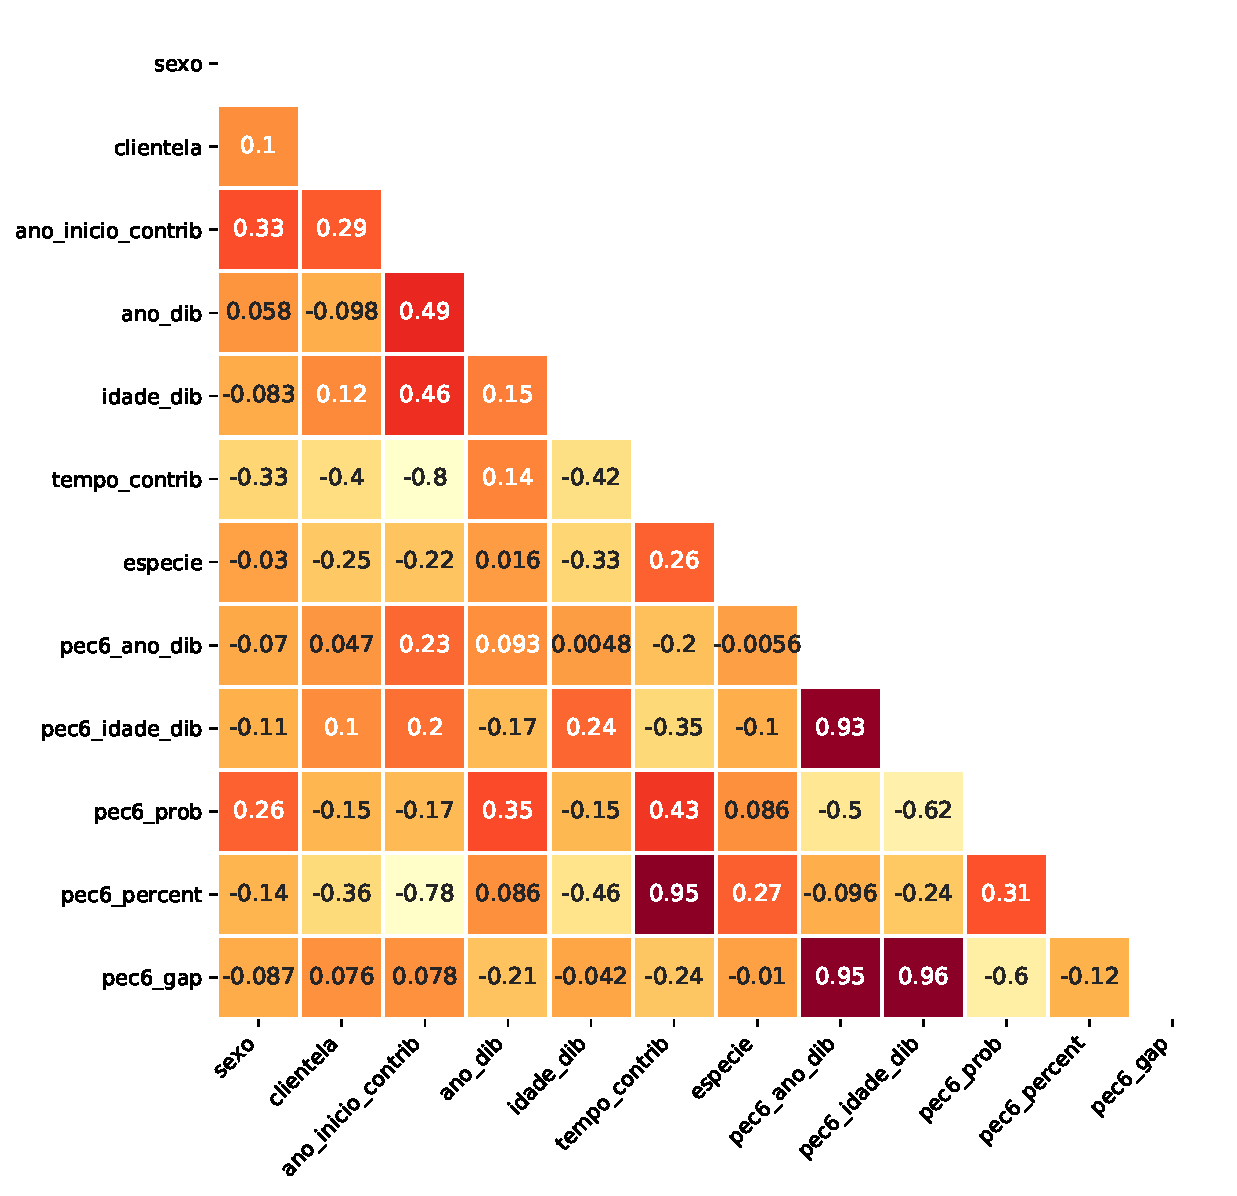
\includegraphics[width=\textwidth]{figs/cap05_corr_matrix.pdf}
%    \caption*{\footnotesize{Fonte: Elaborado pelo autor}}
%    \label{fig:cap05:matrixcorr}
%\end{figure}

\section{Considerações Finais}\label{cap05:conclusoes}

No presente estudo foram realizadas análises acerca dos impactos que a reforma da previdência prevista pela PEC 06/2019 poderia causar no cenário previdenciário nacional, avaliando a série histórica de concessões de aposentadorias entre os anos 1995 e 2016. Nesse contexto, os resultados demonstraram que aproximadamente 78,66\% das aposentadorias concedidas no período analisado não atendem as regras previstas na PEC, fazendo-se necessário um acréscimo em anos de contribuição, ou espera, para que os beneficiários tenham acesso a essas aposentadorias. Paralelamente, foi relatada a dificuldade que os trabalhadores, possivelmente, enfrentariam perante ao novo sistema proposto, uma vez que haverá a necessidade desses manterem-se formais em um mercado de trabalho que não lhe garante total estabilidade.

Adicionalmente, considerando a sobrevida dos aposentados, estimou-se que aproximadamente 6,49\% dos trabalhadores teriam falecido antes de ter acesso ao seu benefício e que 509.763 homens e 78.453 mulheres teriam probabilidade abaixo de 30\% de estarem vivos. Além disso, foi calculado o percentual de repasse que os beneficiários receberiam considerando a regra dos 60\% + 2\% por ano trabalhado, observando que apenas 3\% dos trabalhadores teriam acesso a média integral de todos seus salários, demonstrando a clara dificuldade que as novas regras implicarão para os trabalhadores gozarem desse benefício. 

É evidente que caso as regras previstas pela PEC 06/2019 já estivessem em vigor desde o primeiro ano analisado, o cenário resultante seria diferente do estipulado pelos resultados, afinal, tais regras estimulariam os trabalhadores a terem um perfil diferente no mercado de trabalho. No entanto, é valido considerar os principais desafios que a proposta apresentará para a população, como forma de refletir se essa é melhor alternativa para solucionar o atual problema existente no regime previdenciário nacional.
